\documentclass[a4paper, 12pt]{article}

% ===== 宏包 =====
\usepackage[UTF8]{ctex}               % 中文支持
\usepackage[T1]{fontenc}              % T1 编码，提供直引号等字形
\usepackage[margin=2.5cm]{geometry}   % 页边距
\usepackage{amsmath, amssymb}         % 数学公式
\usepackage{booktabs}                 % 三线表
\usepackage{graphicx}                 % 插图
\usepackage{xcolor}                   % 颜色（需在 listings 之前）
\usepackage{listings}                 % 代码块
\usepackage{textcomp}                % 提供直引号等 TS1 符号
\usepackage{upquote}                 % 代码里的单引号排成直引号，而非弯引号
\usepackage{titlesec}                 % 标题样式
\usepackage{fancyhdr}                 % 页眉页脚
\usepackage{hyperref}                 % 超链接（最后加载）

% ===== 配色：蓝白主题 =====
\definecolor{primary}{HTML}{1F5FA8}   % 主蓝
\definecolor{accent}{HTML}{4A90D9}    % 浅蓝
\definecolor{bgblue}{HTML}{F0F6FC}    % 极浅蓝背景

% ===== 标题样式 =====
\titleformat{\section}{\Large\bfseries\color{primary}}{\thesection}{0.8em}{}
\titleformat{\subsection}{\large\bfseries\color{accent}}{\thesubsection}{0.8em}{}

% ===== 页眉页脚 =====
\pagestyle{fancy}
\fancyhf{}
\fancyhead[L]{\small\color{primary}系统开发工具基础 · 第一周实验报告}
\fancyhead[R]{\small\color{primary}陆立庭 · 25120014018}
\fancyfoot[C]{\small\color{primary}\thepage}
\renewcommand{\headrulewidth}{0.6pt}
\renewcommand{\headrule}{\color{accent}\hrule width\headwidth height\headrulewidth}

% ===== 代码块样式 =====
\lstset{
  basicstyle=\ttfamily\small,
  breaklines=true,
  frame=single,
  rulecolor=\color{accent},
  backgroundcolor=\color{bgblue},
  columns=fullflexible,
  upquote=true,
  showstringspaces=false,
  commentstyle=\color{gray},
  keywordstyle=\color{primary},
  stringstyle=\color{teal},
}

% ===== 超链接样式 =====
\hypersetup{
  colorlinks=true,
  linkcolor=primary,
  urlcolor=accent,
  citecolor=primary,
}

\title{\textbf{\color{primary}系统开发工具基础\quad 第一周实验报告}}
\author{陆立庭\ -\ 25120014018}
\date{2026 年 8 月}

\begin{document}

\maketitle
\vspace{-0.5em}
\noindent{\color{primary}\rule{\textwidth}{1pt}}

\begin{abstract}
本报告围绕第一周四个实验题目展开，覆盖命令行文件与目录操作、Shell 脚本与文本处理、Git 分支管理与冲突解决、以及 \LaTeX{} 排版与交叉引用四大主题。报告按“题目分析与知识点总结”“遇到的问题与解决方法”“实验总结”三个部分组织，并在文末附上本次实验的 GitHub 仓库链接与提交记录截图。
\end{abstract}

\tableofcontents
\newpage

% ============================================================
\section{实验题目分析与知识点总结}
% ============================================================

\subsection{题目一：命令行文件与目录操作}

\textbf{题目分析}：完全使用命令行完成目录与文件的创建、查看与复制，重点考察对基础命令的掌握，以及隐藏文件、文件名含空格等细节的处理。

\textbf{知识点}：
\begin{itemize}
  \item \texttt{mkdir -p} 递归建目录；\texttt{echo -e}/\texttt{printf} 写多行内容；\texttt{touch} 建空文件。
  \item 隐藏文件以 \texttt{.} 开头，用 \texttt{ls -a} 查看；\texttt{pwd} 显示绝对路径；\texttt{ls -la} 长格式含隐藏。
  \item \texttt{cp --parents} 保留相对目录结构；文件名含空格时用引号包裹。
\end{itemize}

关键命令如下：

\begin{lstlisting}[language=bash]
mkdir -p input/docs input/tmp
echo -e "alpha\nbeta" > "input/docs/notes one.txt"
echo hidden > "input/docs/.secret.txt"
touch input/tmp/empty.txt
echo -e "2026-08-25 10:00:00 INFO started\n2026-08-25 10:01:00 INFO done" > input/run.log

pwd            # show absolute path of q01
ls -la input   # long format, incl. hidden files

mkdir -p work/25120014018
find input -name '*.txt' -exec cp --parents {} work/25120014018/ \;
\end{lstlisting}

\subsection{题目二：Shell 脚本与文本处理}

\textbf{题目分析}：编写 \texttt{analyze.sh} 对 CSV 访问日志做统计，要求具备错误处理，并输出 HTTP 5xx 次数最多的前 2 个 \texttt{path} 与平均 \texttt{latency\_ms}。

\textbf{知识点}：
\begin{itemize}
  \item \texttt{\$1} 接收参数；\texttt{[ ! -f "\$1" ]} 判断文件存在；\texttt{>\&2} 写 \texttt{stderr}；\texttt{exit 1} 返回非零退出码。
  \item \texttt{awk -F,} 解析 CSV；\texttt{NR>1} 排除表头；\verb|/^5[0-9][0-9]$/| 匹配 5xx 状态码。
  \item \texttt{sort -k1,1nr -k2,2} 按次数降序、次数相同按 \texttt{path} 字典序；\texttt{head -n 2} 取前二；\texttt{printf "\%.2f"} 保留两位小数。
\end{itemize}

参考实现如下（假设 CSV 列为 \texttt{path, status\_code, latency\_ms}）：

\begin{lstlisting}[language=bash]
#!/bin/bash
# Usage: ./analyze.sh <csv_file_path>
# Assumed CSV columns: path,status_code,latency_ms

if [ ! -f "$1" ]; then
    echo "Error: file $1 not found" >&2
    exit 1
fi

echo "== top-2 paths by HTTP 5xx count =="
awk -F, 'NR>1 && $2 ~ /^5[0-9][0-9]$/ {count[$1]++}
         END { for (p in count) print count[p], p }' "$1" \
  | sort -k1,1nr -k2,2 | head -n 2

echo "== average latency_ms =="
awk -F, 'NR>1 { s += $3; n++ }
         END { if (n > 0) printf "%.2f\n", s/n }' "$1"
\end{lstlisting}

\subsection{题目三：Git 分支管理与冲突解决}

\textbf{题目分析}：初始化仓库后，从 \texttt{main} 分别创建 \texttt{feature-a}、\texttt{feature-b}，各自修改 \texttt{config.txt} 同一行并提交，再依次合并；第二次合并产生冲突，需保留 \texttt{mode=safe} 并追加 \texttt{note=reviewed}。

\textbf{知识点}：
\begin{itemize}
  \item \texttt{git init}/\texttt{add}/\texttt{commit} 初始化与提交；\texttt{git switch -c} 创建并切换分支。
  \item \texttt{git merge} 合并；冲突处用 \texttt{<<<<<<<}、\texttt{=======}、\texttt{>>>>>>>} 标记，手工编辑后 \texttt{add}+\texttt{commit}。
  \item \texttt{git status} 确认工作区干净；\texttt{git log --all --graph --decorate --oneline} 图形化查看历史。
\end{itemize}

关键命令如下：

\begin{lstlisting}[language=bash]
git init
echo "mode=normal" > config.txt
git add config.txt && git commit -m "init config"

git switch -c feature-a
echo "mode=safe" > config.txt
git commit -am "feature-a: mode=safe"

git switch -c feature-b main     # create from initial main
echo "mode=fast" > config.txt
git commit -am "feature-b: mode=fast"

git switch main
git merge feature-a
git merge feature-b              # conflict, resolve manually
# keep mode=safe, add note=reviewed
git add config.txt && git commit -m "merge feature-b, keep mode=safe"

git status                       # confirm working tree is clean
git log --all --graph --decorate --oneline
\end{lstlisting}

\subsection{题目四：\LaTeX{} 排版与交叉引用}

\textbf{题目分析}：加入带编号与 \texttt{label} 的公式、带 \texttt{caption} 与 \texttt{label} 的 2×2 表格，并在正文中交叉引用；用 \texttt{latexmk -pdf -halt-on-error} 生成 PDF 且无 \texttt{??}。

\textbf{知识点}：
\begin{itemize}
  \item \texttt{equation} 环境 + \texttt{\textbackslash label\{\}} + \texttt{\textbackslash eqref\{\}}（需 \texttt{amsmath}）。
  \item \texttt{table} 浮动体 + \texttt{tabular} + \texttt{\textbackslash caption} + \texttt{\textbackslash label}，正文用 \texttt{\textbackslash ref} 引用。
  \item \texttt{latexmk -pdf -halt-on-error} 自动多轮编译；交叉引用需\textbf{连续编译两次}消除 \texttt{??}。
\end{itemize}

以下公式与表格即本报告按题目要求所演示的带标签实例。平均时延按公式~\eqref{eq:mean-latency} 计算：

\begin{equation}
  \bar{L} = \frac{1}{n} \sum_{i=1}^{n} L_i
  \label{eq:mean-latency}
\end{equation}

第一周四个题目的主题对照见表~\ref{tab:overview}：

\begin{table}[h]
  \centering
  \begin{tabular}{ll}
    \toprule
    \textbf{题目} & \textbf{核心主题} \\
    \midrule
    题目一 & 命令行文件与目录操作 \\
    题目二 & Shell 脚本与文本处理 \\
    题目三 & Git 分支管理与冲突解决 \\
    题目四 & \LaTeX{} 排版与交叉引用 \\
    \bottomrule
  \end{tabular}
  \caption{第一周实验题目主题对照表}
  \label{tab:overview}
\end{table}

% ============================================================
\section{实验遇到的问题与解决方法}
% ============================================================

\subsection{问题一：Ubuntu 虚拟机登录密码遗忘}

\textbf{问题描述}：登录 Ubuntu 虚拟机时忘记用户密码，无法进入系统。

\textbf{解决方法}：开机进入 GRUB 引导菜单，选择 Advanced options 中的 recovery mode（进入 root 恢复界面），在 root shell 中执行 \texttt{passwd <用户名>} 重置密码，重启后即可正常登录。

\subsection{问题二：第二题脚本输出结果难以判断是否正确}

\textbf{问题描述}：\texttt{analyze.sh} 输出的 Top-2 \texttt{path} 与平均 \texttt{latency\_ms} 缺少对照，无法确认统计结果是否正确。

\textbf{解决方法}：构造小规模测试 CSV，先手工/心算得到预期结果，再与脚本输出比对；同时用 \texttt{awk} 逐步输出中间结果，核对表头是否已排除、5xx 匹配是否无误。

\subsection{问题三：第三题 Git 分支合并冲突}

\textbf{问题描述}：合并 \texttt{feature-b} 时，因该分支与 \texttt{feature-a} 修改了 \texttt{config.txt} 的同一行，Git 报合并冲突，无法自动完成合并。

\textbf{解决方法}：打开冲突文件，手工编辑冲突标记，保留 \texttt{mode=safe} 并追加 \texttt{note=reviewed}，随后 \texttt{git add} 与 \texttt{git commit} 完成合并，并用 \texttt{git status} 确认工作区干净。

\subsection{问题四：\LaTeX{} 中文页眉页脚设计}

\textbf{问题描述}：默认 \texttt{article} 类没有页眉页脚，且想在报告中显示中文页眉页脚时，遇到中文支持与格式设置的配合问题。

\textbf{解决方法}：加载 \texttt{fancyhdr} 宏包并配合 \texttt{ctex}，用 \texttt{\textbackslash fancyhead} 与 \texttt{\textbackslash fancyfoot} 设置中文页眉页脚，再通过 \texttt{\textbackslash renewcommand\{\textbackslash headrule\}} 定制页眉横线的颜色与粗细。

% ============================================================
\section{实验总结}
% ============================================================

通过本周实验，我系统地掌握了以下内容：

\begin{itemize}
  \item \textbf{命令行基础}：熟练使用 \texttt{mkdir}、\texttt{echo}、\texttt{touch}、\texttt{ls}、\texttt{find}、\texttt{cp} 等命令，并理解隐藏文件与文件名含空格的处理技巧。
  \item \textbf{Shell 脚本与文本处理}：掌握参数接收、错误处理与退出码，能借助 \texttt{awk}、\texttt{sort}、\texttt{head} 及管道完成日志统计。
  \item \textbf{Git 版本控制}：熟悉分支的创建、切换与合并，理解合并冲突的产生原因与解决流程。
  \item \textbf{\LaTeX{} 排版}：学会中文宏包、数学公式、表格、交叉引用与页眉页脚设计，并了解需多次编译生成正确引用。
\end{itemize}

这些工具是后续系统开发实践中不可或缺的基础技能，为后续课程与项目开发打下了良好的基础。

% ============================================================
\section{附录：GitHub 链接与提交记录}
% ============================================================

本次实验代码已提交至 GitHub 仓库，地址如下：

\begin{center}
  \url{https://github.com/lyun69965/primary-system-tools.git}
\end{center}

下图为本仓库的 commit 提交记录截图：

\begin{figure}[h]
  \centering
  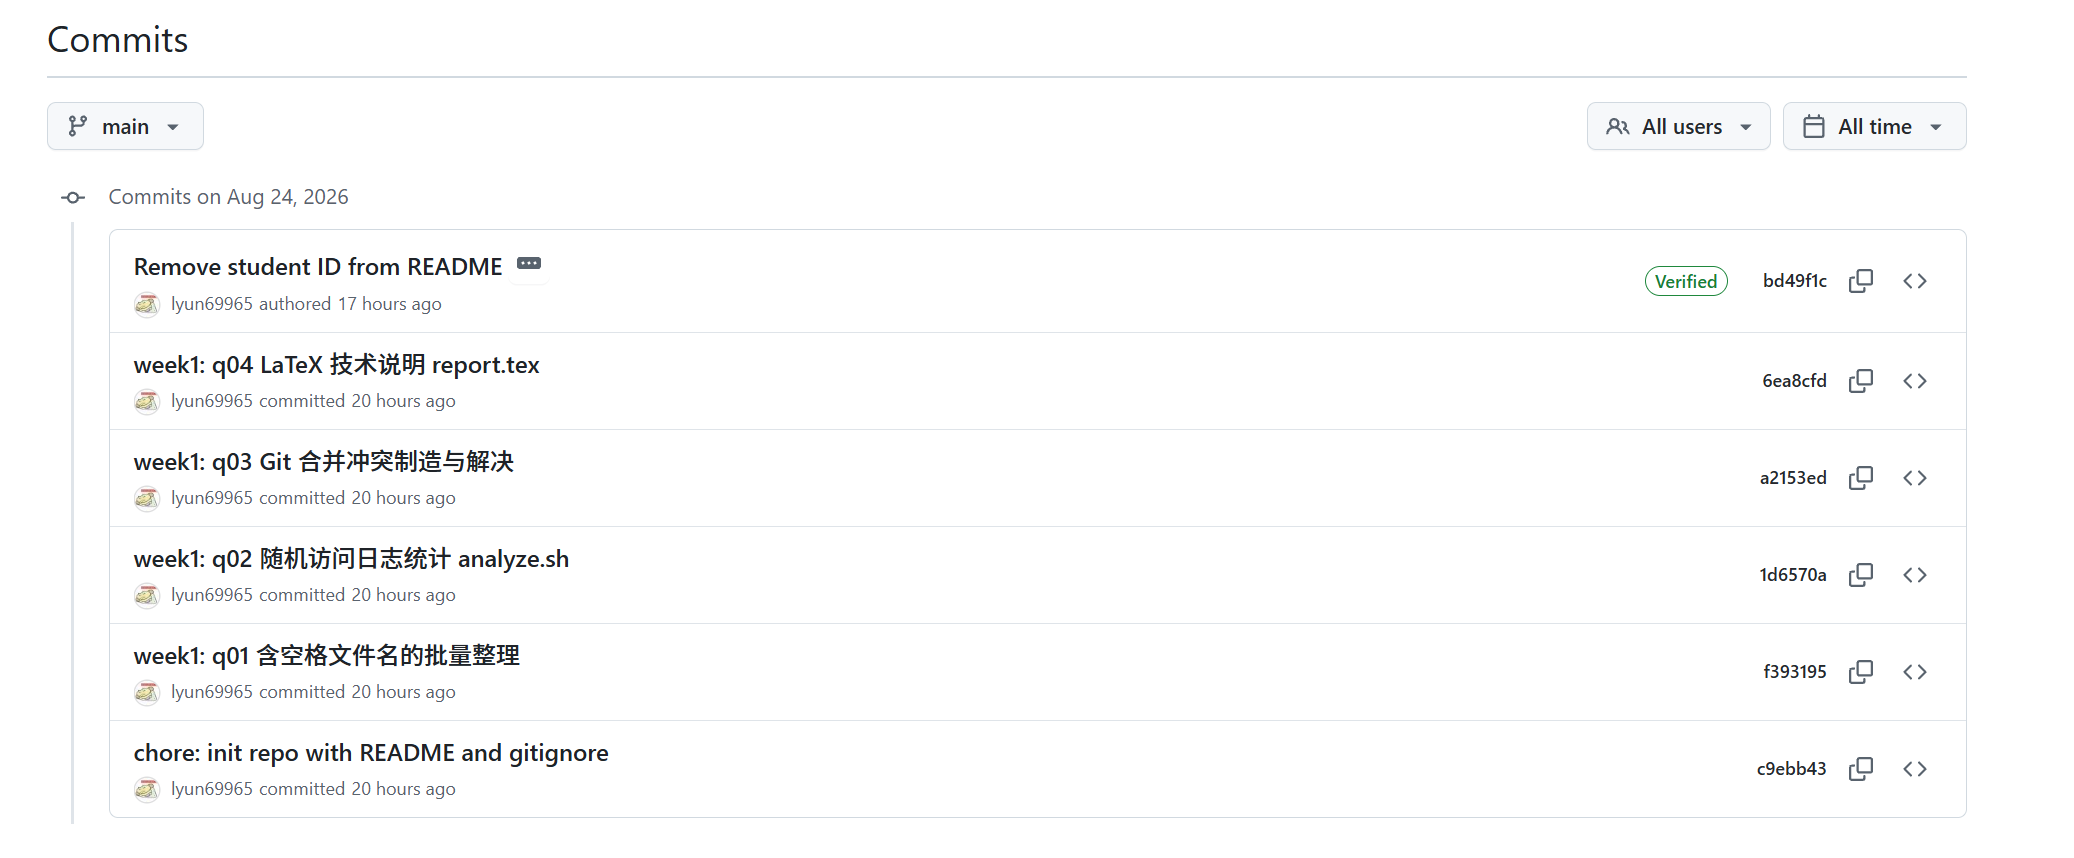
\includegraphics[width=0.85\textwidth]{commit.png}
  \caption{GitHub 仓库 commit 提交记录}
  \label{fig:commit}
\end{figure}

\end{document}
